% === Cours de Java

\section{Organiser le code}

\leconwithabstract{Dans une application r�elle, la taille des programmes impose une organisation rigoureuse}

\begin{frame}{Le groupement en package}
L'\emph{API} (Application Programming Interface) d�signe la biblioth�que standard Java
\begin{itemize}
\item Elle contient des \emph{milliers} de classes
\item Elles sont regroup�es en \emph{package}
\end{itemize}
\begin{center}
  %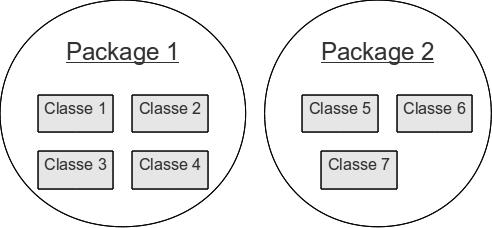
\includegraphics[scale=.6]{../img/package}
\end{center}
\end{frame}

\begin{frame}{La notion de package}
Un \emph{package}
\begin{itemize}
\item Regroupe les classes li�es
\item Permet l'unicit� des noms de classe
  \begin{itemize}
    \item nom complet / qualifi�: {\small \java|monPackage.MaClasse|}
  \end{itemize} 
\end{itemize} 
\bigskip
Nom d'un package
  \begin{itemize}
    \item identifieurs s�par�s par des points \java|.|
    \item tout en minuscules
    \item adresse internet invers�e (unicit�)
    \item ex: {\small \java|be.heb.esi.java1|}, {\small \java|org.apache.struts.action|}
  \end{itemize} 
\end{frame}

\begin{frame}[fragile]{Utilisation}
Pour utiliser une classe 
\begin{itemize}
\item mettre le nom \emph{qualifi�} (complet)
\begin{Java}
  java.util.Calendar now = java.util.Calendar.getInstance();
\end{Java}
\item ou utiliser \java{import} qui cr�e un raccourci
\begin{Java}[basicstyle=\scriptsize]
  import java.util.Calendar;
  public Test {
  ...
    Calendar now = Calendar.getInstance();
  ...
  }
\end{Java}
\item Cas particulier : le package \java|java.lang| est import� implicitement
  \begin{itemize}
  \item Exemple : on peut tout de suite �crire
  \begin{Java}
  double racine = Math.sqrt(1.21);
  \end{Java}
  \end{itemize}
\end{itemize}
\end{frame}

\begin{frame}{Utilisation}
Comment savoir comment utiliser les classes et m�thodes ? En lisant la \emph{javadoc}
%\begin{center}
%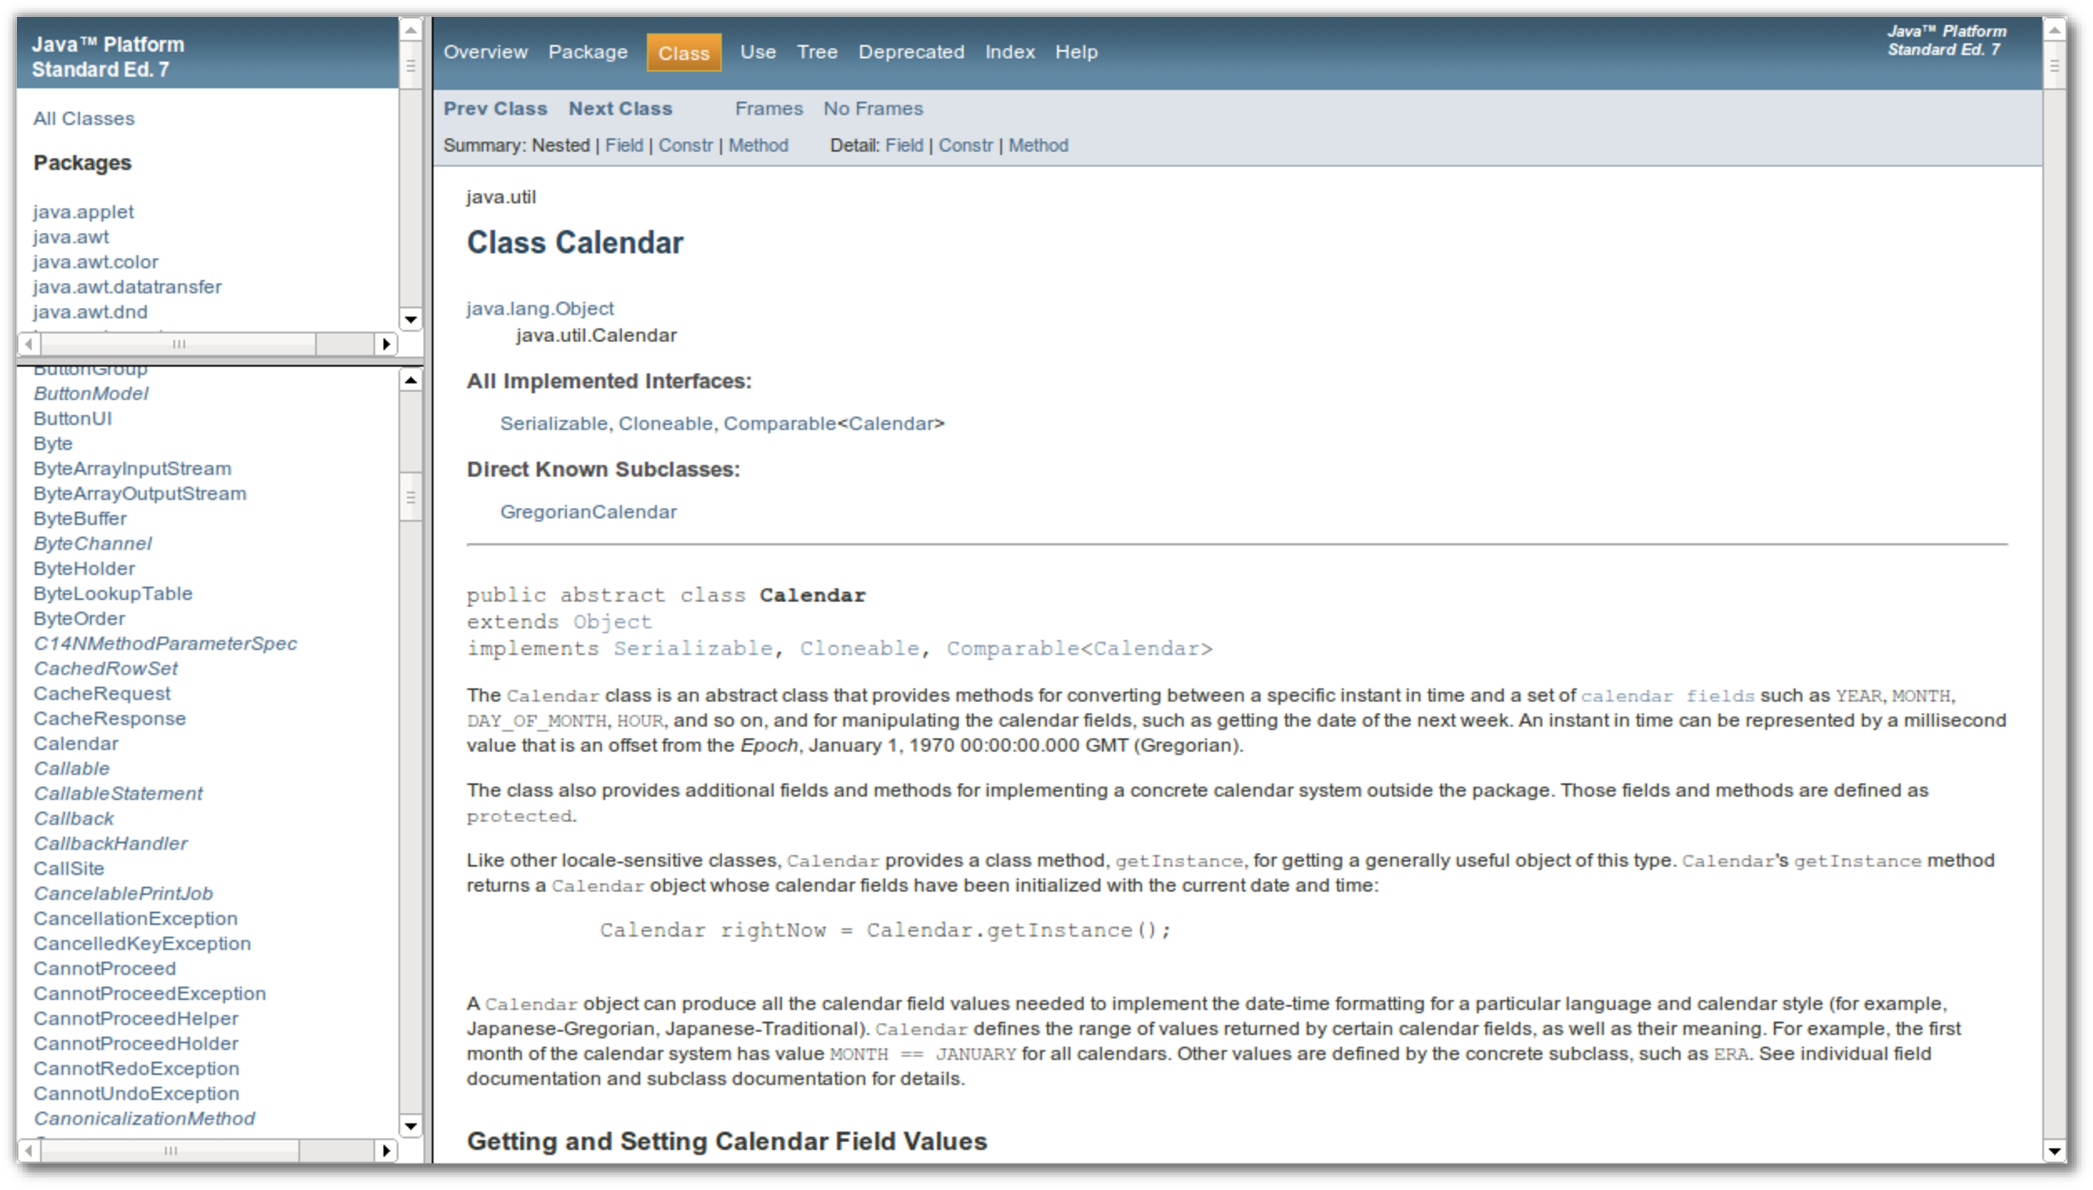
\includegraphics[scale=.28]{../img/api}
%\\ \scriptsize{\textit{(http://download.oracle.com/javase/7/docs/api/)}}
%\end{center}
\end{frame}

\begin{frame}{Utilisation}
On peut y lire le nom du package 
\begin{center}
%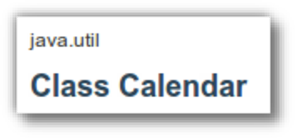
\includegraphics[scale=.6]{../img/api-package}
\end{center}
et la description de la m�thode
%\begin{center}
%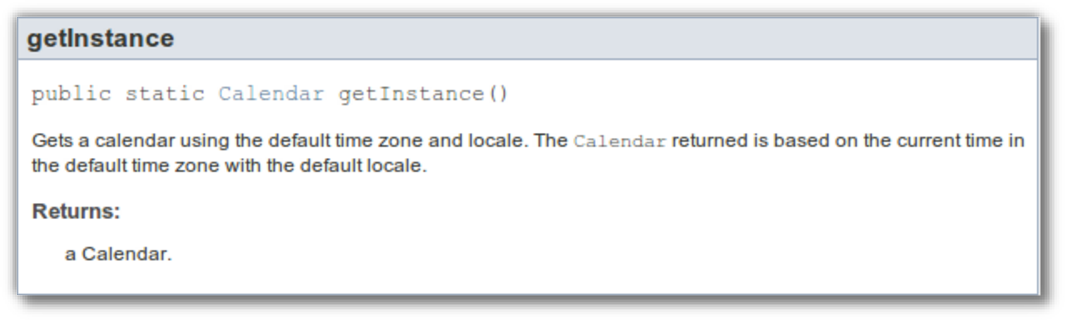
\includegraphics[scale=.6]{../img/api-methode}
%\\{\small \textit{On verra comment produire une \emph{javadoc} similaire pour son code}}
%\end{center}
\end{frame}

\begin{frame}[fragile]{Cr�er ses packages}
Pour placer une classe dans un package, la commande est \java|package nom_package;|
  \begin{itemize}
  \item Doit �tre la \emph{premi�re instruction} du fichier 
  \item Exemple :
\begin{Java}
package be.heb.esi.java1;
public class Test { 
  // Nom complet : be.heb.esi.java1.Test
}
\end{Java}
  \end{itemize}
\end{frame}

\begin{frame}[fragile]{Cr�er ses packages}
Qu'est-ce qui va changer en pratique ?
\begin{itemize}
\item La compilation ne change pas : 
 \begin{Java}
 javac NomClasse.java
 \end{Java}
\item L'ex�cution change : 
 \begin{Java}
 java nomPackage.NomClasse
 \end{Java}
\item Contraintes sur l'endroit o� placer le \emph{bytecode}
  \begin{itemize}
  \item Li� � la notion de \emph{CLASSPATH} 
  \item Sera d�taill� au laboratoire
  \end{itemize}
\end{itemize}
\end{frame}

\begin{frame}{R�utiliser du code}
Si on doit coder quelque chose, c'est \emph{peut-�tre d�j� fait}
\begin{itemize}
\item $\Longrightarrow$ autant le r�utiliser
  \begin{itemize}
  \item Gain de temps
  \item Probablement mieux �crit
  \end{itemize}
\item Importance de \emph{connaitre l'API}
\\(en tout cas les classes principales)
\end{itemize}
\end{frame}


